\documentclass[10pt,twocolumn]{article}
\usepackage[letterpaper,landscape,hmargin=1in,top=1in,bottom=1in]{geometry}
\usepackage[utf8]{inputenc}
\usepackage{lmodern}
%\usepackage{fourier}
\usepackage[T1]{fontenc}
%\usepackage{hyperref}
\usepackage[hidelinks]{hyperref}
\usepackage{graphicx}
\usepackage{circledsteps}
\usepackage{amsmath}
\usepackage[french]{babel}
\frenchbsetup{StandardLists=true}
\usepackage{enumitem}
\usepackage{microtype}

%\usepackage{layout}
%\usepackage{lipsum}
%\usepackage{showframe}

\title{Devoir \no 2\thanks{IFT 1575 - Modèles de recherche opérationnelle - Université de Montréal - Hiver~2020~- Jean-Yves \textsc{Potvin}}}
\author{Jeanne \textsc{Laflamme} \and Alexandre \textsc{Pachot}}

\setcounter{tocdepth}{1}
\usepackage{tocloft}
\renewcommand{\cftsecleader}{\cftdotfill{\cftdotsep}}

\renewcommand\thesubsection{(\alph{subsection})}

%\setlength{\columnsep}{.2in}

\begin{document}
	%\layout
	
	\maketitle
	\renewcommand{\contentsname}{}
	\tableofcontents
	%\lipsum
	
	\section*{Question 1}
\addcontentsline{toc}{section}{Question 1}

\emph{Trouver des valeurs pour $a$, $b$, $c$ et $d$ telles que : $x_7$ est variable d’entrée, $x_5$ est variable de sortie\dots}
\begin{center}
	\renewcommand{\arraystretch}{1.5}
	\begin{tabular}{|c|cccccccc|c|}
		\hline
		v.d.  & $x_1$ & $x_2$ & $x_3$ & $x_4$ & $x_5$ & $x_6$ & $x_7$ & $-z$ & t.d. \\ \hline
		$x_3$ &   3   &       &   1   &  $a$  &       & $-1$  &       &      &  1   \\
		$x_2$ &   4   &   1   &       & $-1$  &       &   2   &  $b$  &      &  6   \\
		$x_5$ & $-1$  &       &       &   2   &   1   &  $c$  &   4   &      &  5   \\ \hline
		$-z$  &   2   &       &       &   3   &       &   2   &  $d$  &  1   &  25  \\ \hline
	\end{tabular}
\end{center}

Afin que $x_5$ soit variable de sortie, on doit avoir $min \{\frac{5}{4}, \frac{6}{b}\}$ = $\frac{5}{4}$ ce qui implique que $\frac{5}{4} < \frac{6}{b}$ et donc que $b < \frac{24}{5}$. On peut alors effectuer on pivot pour obtenir le tableau suivant:

\begin{center}
	\renewcommand{\arraystretch}{1.5}
	\begin{tabular}{|c|cccccccc|c|}
		\hline
		v.d.  &      $x_1$      & $x_2$ & $x_3$ &      $x_4$       &     $x_5$      &      $x_6$       & $x_7$ & $-z$ &       t.d.        \\ \hline
		$x_3$ &        3        &       &   1   &       $a$        &                &        $-1$        &       &      &         1         \\
		$x_2$ & $4+\frac{b}{4}$ &   1   &       & $-1-\frac{b}{2}$ & $-\frac{b}{4}$ & $2-\frac{bc}{4}$ &       &      & $6-\frac{5b}{4}$  \\
		$x_7$ & $-\frac{1}{4}$  &       &       &  $\frac{1}{2}$   & $\frac{1}{4}$  &  $\frac{c}{4}$   &   1   &      &   $\frac{5}{4}$   \\ \hline
		$-z$  & $2+\frac{d}{4}$ &       &       & $3-\frac{d}{2}$  & $-\frac{d}{4}$ & $2-\frac{cd}{4}$ &       &  1   & $25-\frac{5d}{4}$ \\ \hline
	\end{tabular}
\end{center}

\emph{\dots et après une itération du simplexe on se retrouve dans une situation où on a :}

\subsection{Une solution optimale unique}

Afin que la solution soit optimale, tous les coût doivent être positifs. Les variables $a,b,c,d$ doivent donc respecter les contraintes suivantes:
\begin{enumerate}[label=(\arabic*),itemsep=1pt]
	\item $2 + \frac{d}{4} > 0 \Rightarrow d > -8$
	\item $3 - \frac{d}{2} > 0 \Rightarrow d < 6$
	\item $ - \frac{d}{4} > 0 \Rightarrow d < 0$
	\item $2 - \frac{cd}{4} > 0 \Rightarrow cd < 8$
\end{enumerate}

On peut donc choisir par exemple $a = 1$, $b=4$, $c=2$ et $d=-4$ pour obtenir le tableau suivant qui est optimale:
	
\begin{center}
	\renewcommand{\arraystretch}{1.5}
	\begin{tabular}{|c|cccccccc|c|}
		\hline
		v.d.  &     $x_1$      & $x_2$ & $x_3$ &     $x_4$     &     $x_5$     &     $x_6$     & $x_7$ & $-z$ &     t.d.      \\ \hline
		$x_3$ &       3        &       &   1   &       1       &               &     $-1$      &       &      &       1       \\
		$x_2$ &       5        &   1   &       &     $-3$      &     $-1$      &               &       &      &       1       \\
		$x_7$ & $-\frac{1}{4}$ &       &       & $\frac{1}{2}$ & $\frac{1}{4}$ & $\frac{1}{2}$ &   1   &      & $\frac{5}{4}$ \\ \hline
		$-z$  &       1        &       &       &       5       &       1       &       4       &       &  1   &      30       \\ \hline
	\end{tabular}
\end{center}

\subsection{Une solution optimale qui n’est pas unique}
Pour avoir une solution optimale qui n’est pas unique, on doit avoir une des variables indépendantes qui a un coût nul. En fixant par exemple $\bar{c}_1$ à zéro, on obtient la contrainte:
\begin{enumerate}[label=(\arabic*),itemsep=1pt]
	\setcounter{enumi}{4}
	\item  $2 + \frac{d}{4} = 0 \Rightarrow d = -8$
\end{enumerate}

En plus des contraintes (2), (3), (4). On peut alors choisir $a = 1$, $b=4$, $c=2$ et $d=-8$ pour obtenir le tableau suivant qui est optimale mais non-unique car on pourrait effectuer un pivot avec $x_1$ comme variable d’entrée pour obtenir une autre solution:
	
\begin{center}
	\renewcommand{\arraystretch}{1.5}
	\begin{tabular}{|c|cccccccc|c|}
		\hline
		v.d.  &     $x_1$      & $x_2$ & $x_3$ &     $x_4$     &     $x_5$     &     $x_6$     & $x_7$ & $-z$ &     t.d.      \\ \hline
		$x_3$ &       3        &       &   1   &       1       &               &     $-1$      &       &      &       1       \\
		$x_2$ &       5        &   1   &       &     $-3$      &     $-1$      &               &       &      &       1       \\
		$x_7$ & $-\frac{1}{4}$ &       &       & $\frac{1}{2}$ & $\frac{1}{4}$ & $\frac{1}{2}$ &   1   &      & $\frac{5}{4}$ \\ \hline
		$-z$  &                &       &       &       7       &       2       &       6       &       &  1   &      35       \\ \hline
	\end{tabular}
\end{center}

\subsection{Un problème non borné inférieurement}
Afin que le problème soit non borné inférieurement, on doit avoir une variable dont le coût est négatif et dont les coefficients dans toutes les contraintes sont négatifs. Dans ce cas, on pourra augmenter cette variable indéfiniment et donc faire diminuer l’objectif autant qu’on veut. Si on choisi par exemple la variable $x_6$, les contraintes suivantes sur $a$,$b$,$c$ et $d$ doivent être satisfaites :
\begin{enumerate}[label=(\arabic*),itemsep=1pt]
	\setcounter{enumi}{5}
	\item $2 - \frac{bc}{4} \geq 0 \Rightarrow bc \geq 8$
	\item $\frac{c}{4} \geq 0 \Rightarrow  c \leq 0$
	\item $2 - \frac{cd}{4} < 0 \Rightarrow cd > 8$
\end{enumerate}

On peut alors choisir $a = 1$, $b = -4$, $c = -2$ et $d = -8$ pour obtenir le tableau suivant:
	
\begin{center}
	\renewcommand{\arraystretch}{1.5}
	\begin{tabular}{|c|cccccccc|c|}
		\hline
		v.d.  &     $x_1$      & $x_2$ & $x_3$ &     $x_4$     &     $x_5$     &     $x_6$      & $x_7$ & $-z$ &     t.d.      \\ \hline
		$x_3$ &       3        &       &   1   &       1       &               &      $-1$      &       &      &       1       \\
		$x_2$ &       3        &   1   &       &       2       &       1       &                &       &      &       1       \\
		$x_7$ & $-\frac{1}{4}$ &       &       & $\frac{1}{2}$ & $\frac{1}{4}$ & $-\frac{1}{2}$ &   1   &      & $\frac{5}{4}$ \\ \hline
		$-z$  &                &       &       &       7       &       2       &      $-2$      &       &  1   &      35       \\ \hline
	\end{tabular}
\end{center}

	\section*{Question 2}
\addcontentsline{toc}{section}{Question 2}
\setcounter{subsection}{0}

\emph{Démontrer qu’il ne peut exister de solution de base réalisable où $x_{1j}$ et $x_{2j}$ sont toutes les deux variables de base, quel que soit $j = 1, \dots, n$.}

On a le tableau initial suivant :

\begin{center}
	\renewcommand{\arraystretch}{1.5}
	\begin{tabular}{|c| ccccccccc|c|}
		\hline
		v.d. & $x_{11}$ & $x_{21}$  & $\cdots$ & $x_{1j}$ & $x_{2j}$  & $\cdots$ & $x_{1n}$ & $x_{2n}$  & $-z$ &   t.d.   \\ \hline
		     & $a_{11}$ & $-a_{11}$ & $\cdots$ & $a_{1j}$ & $-a_{1j}$ & $\cdots$ & $a_{1n}$ & $-a_{1n}$ &      &  $b_1$   \\
		     & $a_{21}$ & $-a_{21}$ & $\cdots$ & $a_{2j}$ & $-a_{2j}$ & $\cdots$ & $a_{2n}$ & $-a_{2n}$ &      &  $b_2$   \\
		     & $\vdots$ & $\vdots$  & $\ddots$ & $\vdots$ & $\vdots$  & $\ddots$ & $\vdots$ & $\vdots$  &      & $\vdots$ \\
		     & $a_{m1}$ & $-a_{m1}$ & $\cdots$ & $a_{mj}$ & $-a_{mj}$ & $\cdots$ & $a_{mn}$ & $-a_{mn}$ &      &  $b_m$   \\ \hline
		$-z$ & $c_1$    &  $-c_1$   & $\cdots$ &  $c_j$   &  $-c_j$   & $\cdots$ &  $c_n$   &  $-c_n$   &  1   &          \\ \hline
	\end{tabular}
\end{center}

Afin de rendre $x_{1j}$ variable indépendante, on doit avoir un 1 vis-à-vis de $x_{1j}$ dans une des contraintes. On peut supposer sans perte de généralité qu’il s’agit de la première contrainte. On doit alors diviser la première ligne du tableau par $a_{1j}$:

\begin{center}
	\renewcommand{\arraystretch}{1.5}
	\begin{tabular}{|c|ccccccccc|c|}
		\hline
		v.d. &        $x_{11}$         &         $x_{21}$         & $\cdots$ & $x_{1j}$ & $x_{2j}$  & $\cdots$ &        $x_{1n}$         &         $x_{2n}$         & $-z$ &          t.d.          \\ \hline
		     & $\frac{a_{11}}{a_{1j}}$ & $-\frac{a_{11}}{a_{1j}}$ & $\cdots$ &    1     &   $-1$    & $\cdots$ & $\frac{a_{1n}}{a_{1j}}$ & $-\frac{a_{1n}}{a_{1j}}$ &      & $\frac{b_{1}}{a_{1j}}$ \\
		     &        $a_{21}$         &        $-a_{21}$         & $\cdots$ & $a_{2j}$ & $-a_{2j}$ & $\cdots$ &        $a_{2n}$         &        $-a_{2n}$         &      &         $b_2$          \\
		     &        $\vdots$         &         $\vdots$         & $\ddots$ & $\vdots$ & $\vdots$  & $\ddots$ &        $\vdots$         &         $\vdots$         &      &        $\vdots$        \\
		     &        $a_{m1}$         &        $-a_{m1}$         & $\cdots$ & $a_{mj}$ & $-a_{mj}$ & $\cdots$ &        $a_{mn}$         &        $-a_{mn}$         &      &         $b_m$          \\ \hline
		$-z$ &          $c_1$          &          $-c_1$          & $\cdots$ &  $c_j$   &  $-c_j$   & $\cdots$ &          $c_n$          &          $-c_n$          &  1   &                        \\ \hline
	\end{tabular}
\end{center}

On peut maintenant effectuer un pivot pour obtenir:

\begin{center}
	%\begin{small}
	\renewcommand{\arraystretch}{1.5}
	\begin{tabular}{|c|ccccccccc|c|}
		\hline
		  v.d.   &        $x_{11}$         &         $x_{21}$         & $\cdots$ & $x_{1j}$ & $x_{2j}$ & $\cdots$ &        $x_{1n}$         &         $x_{2n}$         & $-z$ &          t.d.          \\ \hline
		$x_{1j}$ & $\frac{a_{11}}{a_{1j}}$ & $-\frac{a_{11}}{a_{1j}}$ & $\cdots$ &    1     &   $-1$   & $\cdots$ & $\frac{a_{1n}}{a_{1j}}$ & $-\frac{a_{1n}}{a_{1j}}$ &      & $\frac{b_{1}}{a_{1j}}$ \\
		         &     $\bar{a}_{21}$      &     $-\bar{a}_{21}$      & $\cdots$ &          &          & $\cdots$ &     $\bar{a}_{2n}$      &     $-\bar{a}_{2n}$      &      &     $\bar{b}_{2}$      \\
		         &        $\vdots$         &         $\vdots$         & $\ddots$ & $\vdots$ & $\vdots$ & $\ddots$ &        $\vdots$         &         $\vdots$         &      &        $\vdots$        \\
		         &     $\bar{a}_{m1}$      &     $-\bar{a}_{m1}$      & $\cdots$ &          &          & $\cdots$ &     $\bar{a}_{mn}$      &     $-\bar{a}_{mn}$      &      &      $\bar{b}_m$       \\ \hline
		  $-z$   &      $\bar{c}_{1}$      &       $-\bar{c}_1$       & $\cdots$ &          &          & $\cdots$ &       $\bar{c}_n$       &       $-\bar{c}_1$       &  1   &       $\bar{z}$        \\ \hline
	\end{tabular}
	%\end{small}
\end{center}

Dans ce tableau, tous les coefficients de $x_{2j}$ sont zéros sauf dans la première ligne et donc il est impossible de faire entrer $x_{2j}$ dans la base sans faire sortir $x_{1j}$

Ceci démontre qu’il est impossible d’avoir $x_{1j}$ et $x_{2j}$ dans la base en même temps.

	\section{Question 3}
	\section*{Question 4}
\addcontentsline{toc}{section}{Question 4}
\begin{em}
Soit le problème :

\begin{tabular}{@{}rrrrrrrrrrrr@{}}
	Min $z =$ &  $5x_1$ &     &       &     &       & $+$ & $3x_4$ & $-$ & $2x_5$ &     &    \\
	 Sujet à: & $-6x_1$ &     &       & $+$ & $x_3$ & $-$ & $2x_4$ & $+$ & $2x_5$ & $=$ &  $6$ \\
	          & $-3x_1$ & $+$ & $x_2$ &     &       & $+$ & $5x_4$ & $+$ & $3x_5$ & $=$ & $15$
\end{tabular}

Expliquer comment on peut augmenter le tableau optimal afin d’y inclure la variable~$x_6$ sans qu’il soit nécessaire d’appliquer à nouveau l’algorithme du simplexe.
\end{em}

Lorsqu’on résout ce problème avec l’algorithme du simplexe. Le premier tableau est:

\begin{center}
	\renewcommand{\arraystretch}{1.5}
	\begin{tabular}{|c|cccccc|c|}
		\hline
		 v.d.   & $x_{1}$ & $x_{2}$ & $x_{3}$ & $x_{4}$ & $x_{5}$ & $-z$ & t.d. \\ \hline
		$x_{3}$ &  $-6$   &         &    1    &  $-2$   &    2    &      &  6   \\
		$x_{2}$ &  $-3$   &    1    &         &    5    &    3    &      &  15  \\ \hline
		 $-z$   &    5    &         &         &    3    &  $-2$   &  1   &  0   \\ \hline
	\end{tabular}
\end{center}

Dans le tableau initial, les valeurs des colonnes $x_3$ et $x_2$ sont identiques à celles de la matrice identité, ainsi les valeurs de ces deux colonnes dans le tableau optimal sont les valeurs de $B^{-1}$. On a :

\[
B^{-1} = 
\begin{pmatrix}
	-1/4 & 1/2 \\
	-1/4 & 1/6
\end{pmatrix}
\]

Ainsi, une nouvelle variable qui a des coefficients de $-2$ et 6 dans la première et deuxième contrainte aura pour valeur dans le tableau optimal :
\[
\begin{pmatrix}
	-1/4 & 1/2 \\
	-1/4 & 1/6
\end{pmatrix}
\begin{pmatrix}
	-2 \\
	6
\end{pmatrix}
=
\begin{pmatrix}
	7/2 \\
	3/2
\end{pmatrix}
\]

On agit de la même façon pour la valeur de $z$. On prend les valeurs de $z$ des $x_3$ et $x_2$ dans le tableau optimal. Ainsi, on a :
\[
\begin{pmatrix}
3/4 & 1/6 
\end{pmatrix}
\begin{pmatrix}
-2 \\
6
\end{pmatrix}
=
-\frac{1}{2}
\]

Il faut ajouter ce nombre au cout dans l’objectif :
\[1 -\frac{1}{2} = \frac{1}{2}\]

Le tableau optimal avec la nouvelle variable est :

\begin{center}
	\renewcommand{\arraystretch}{1.5}
	\begin{tabular}{|c|ccccccc|c|}
		\hline
		 v.d.   & $x_{1}$ & $x_{2}$ & $x_{3}$ & $x_{4}$ & $x_{5}$ & $x_{6}$ & $-z$ & t.d. \\ \hline
		$x_{5}$ &         &  $1/2$  & $- 1/4$ &    3    &    1    &  $7/2$  &      &  6   \\
		$x_{1}$ &    1    &  $1/6$  & $- 1/4$ &  $4/3$  &         &  $3/2$  &      &  1   \\ \hline
		 $-z$   &         &  $1/6$  &  $3/4$  &  $7/3$  &         &  $1/2$  &  1   &  7   \\ \hline
	\end{tabular}
\end{center}

\emph{En supposant que la variable~$x_6$ représente le niveau d’une certaine activité, que pouvez-vous conclure à propos de cette activité ?}

La valeur de $\bar{c}_6$ est de 1/2, c’est une valeur positive. Si c’était une valeur négative, modifier les variables dépendantes, en faire entrer une pour en faire une autre, ce qui aurait changé la solution. Ce n’est pas le cas. Cette nouvelle activité ne change en rien la solution optimale.

	\section{Question 5}
L’algorithme de branch-and-bound est représenté à la figure~\ref{arbre5}.

\begin{figure}[htb]
	\caption{Algorithme par séparation et évaluation, branch and bound}
	\label{arbre5}
	\centering
	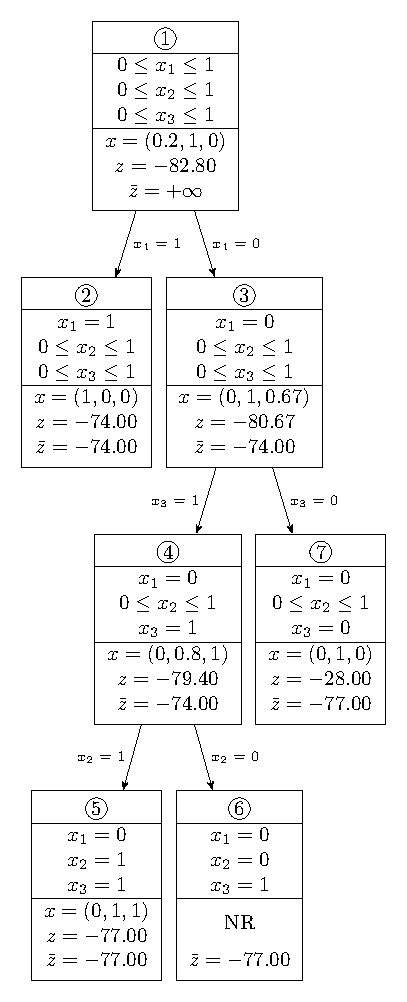
\includegraphics[height=.98\textheight]{question/forest/5.pdf}
\end{figure}

La solution optimale \Circled{1} est $x = (0.2, 1, 0)$ et la valeur de la fonction à minimiser est égale à $-82.80$. Étant donné que $x$ n’est pas une solution entière et que $x_1$ est la seule valeur non entière, nous allons appliquer une contrainte sur sur $x_1$. Soit $x_1 = 1$ , soit $x_1 = 0$. En contraignant $x$ à être égale à 1, on trouve une solution entière : $x = (0.2, 1, 0)$ \Circled{2}. Le meilleur minimum avec une solution passe ainsi de $+\infty$ (pas de solution) à $-74.00$. Étant donné qu’on a trouvé une solution entière, on arrête l’exploration de cette branche pour passer à la contrainte $x_1 = 0$x. Sur cette branche, on trouve une nouvelle solution $x = (0, 1, 0.67)$ \Circled{3}. $x_3$ étant la seule valeur non entière de la solution on va appliquer la contrainte à cette variable. Et ainsi de suite. Il y a trois raisons pour lesquelles on peut arrêter l’exploration d’une branche :
\begin{itemize}
	\item la solution n’est pas réalisable \Circled{6};
	\item la solution est entière \Circled{2} \Circled{5} \Circled{7};
	\item la solution prend une valeur supérieure à une solution entière déjà trouvée ($z \geq \bar{z}$) : cela ne sert à rien d’explorer la branche plus en avant, toutes les solutions entières trouvées seront moins optimales que l’actuelle meilleure solution entière.
\end{itemize}
	
\end{document}
